\section{Ambiente de Contratação Livre}

\subsection{Introdução}

No capítulo passado falamos sobre o ambiente de contratação regulado (ACR), onde as distribuidoras compram energia por meio de leilões, e vendem esta energia para os consumidores. Todo o ACR está sustentado nos leilões. Agora falaremos do ambiente de contratação livre (ACL), onde contratos podem ser negociados livremente entre gerador, comercializador e consumidor. 

O ACL oferece uma maior flexibilidade na negociação de contrato, produtos diferenciados e a possibilidade de gerência de risco. Entretanto, é um mercado onde existe uma maior assimetria de informação e regras muito complexa, principalmente quando se trata do rateio dos custos de transação. Não é qualquer consumidor que pode entrar no ACL, algumas condições devem ser atendidas. Consumidores normais só podem entrar se tiverem uma demanda superior a 3kW. Entretanto, para gerar um incentivo às fontes renováveis, foi permitido que consumidores com demanda superior a 500kW participassem do ACL desde que contratados com renováveis. Além disso, fontes renováveis tem um desconto de $50\%$ na transmissão, permitindo que a energia seja vendida a um preço menor. Em outros países as regras são diferentes, por exemplo, na Europa e na Nova Zelândia todos os consumidores podem escolher de onde compram energia. 

\subsection{O Mercado}

Com a criação do ACL surgiu um novo tipo de agente no mercado, o comercializador. Ele contrata energia de geradores e vende a outros geradores e a consumidores. Sua principal função é reduzir o custo de transação fazendo o casamento entre geradores e consumidores. Além disso, eles oferecem mais liquidez ao mercado e representam seus clientes junto a CCEE. A grande experiência dos comercializadores permite que eles ofereçam produtos diferenciados, como portfólios de renováveis menos ariscados do que a geração de usinas individuais. 

Um consumidor que está no ambiente regulado pode, a qualquer momento, ir para o ambiente livre. No caso contrário, ou seja, um consumidor livre deseja ir para o regulado, a distribuidora é obrigada a aceita-lo. Entretanto, ela pode pedir um tempo de até 5 anos para entrar no leilão e comprar a energia para este novo consumidor. 

Tipicamente, um contrato no ACL tem contém as seguintes informações:

\begin{itemize}
\item Volume contratado e preço,
\item Período de indexação,
\item Submercado de entrega,
\item Responsabilidade pelo risco de mercado,
\item Modulação,
\item Flexibilidades mensais,
\item Sazonalização,
\item Registro na CCEE,
\item Tavas: tetos e pisos,
\item Pagamentos, multas, etc.
\end{itemize}

O ACL ainda não possui uma bolsa de energia, portanto as negociações são feita em balcões. Isso leva a um mercado desorganizado e com muita assimetria de informação. Além disso, não existe uma entidade que ofereça as garantias financeiras asseguradas por uma bolsa de valores. Entretanto, existem alguns esboços de bolsas no Brasil, porém sem grande volume até o momento. 

Como o ACL funciona como um mercado, o preço se da pelo equilibro entre oferta e demanda, obviamente influenciado por alguns fatores externos, como o PLD. Ainda assim, o preço depende da disposição a vender do gerador e da disposição a comprar do consumidor. 

Como dito anteriormente, existe também um ACL incentivado, onde consumidores menores podem participar desde que contratados de renováveis de geração máxima de 30mW. Além disso existe um desconto de $50\%$ na transmissão para estes casos, desconto este que pode chegar até a $100\%$. A figura \ref{fig:aula13_1} mostra como essa vantagem na transmissão pode ser aproveitada. 


\begin{figure}[H]
\begin{centering}
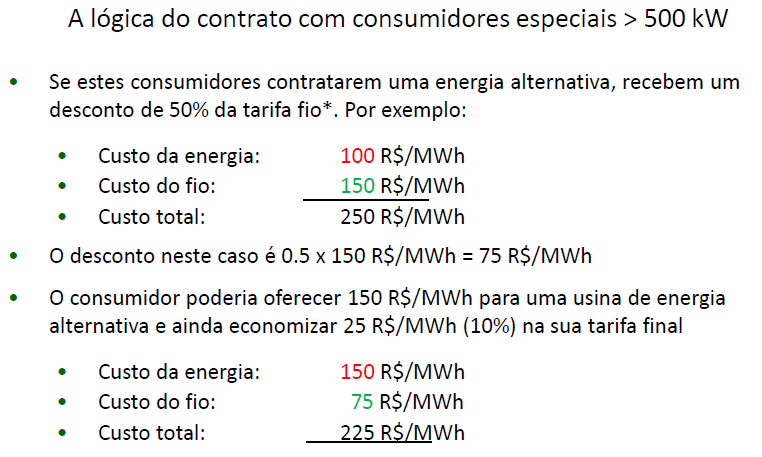
\includegraphics[scale=0.6]{aula13_1}\protect\caption{\label{fig:aula13_1} Vantagens na Transmissão de Renováveis}
\end{centering}
\end{figure}

Cada vez mais os produtos oferecidos pelo ambiente livre estão ficando mais sofisticados. Existem vários tipos de contratos e portfólios oferecidos que visam reduzir o riscos, escapar de efeitos sazonais, e outros. Por exemplo, podemos diversificar entre PCH, biomassa e eólica e ter um fluxo de energia seguro. Imagine uma PCH no sudeste, uma usina de biomassas, também no sudeste e uma eólica no nordeste. Fazendo um portfólio com esses três geradores eliminamos boa parte do risco sazonal, uma vez que suas sazonalidades são complementares. Apesar de tudo isso, observe que no ACL você está sujeito à liquidação de diferenças na CCEE, ou seja, deve contratar uma quantidade de energia, que se ultrapassada será liquidada a PLD. Este tipo de risco não existe quando estamos sob uma distribuidora.  
